% Introduction
\section{Introduction}

%%%%%%

% Cite:
% Wireless networks			#gupta2000capacity
% Wireless sensor networks	#akyildiz2002wireless
% Mobile campus networks 	#hernandez2005comparative
% Mobile gaming community	#cunningham2002optimizing
% Energy-efficient network	#jones2001survey
% Internet of things 			#qin2014software
% Connectivity  			#moscibroda2006complexity
% Density					#wang2015connectivity
% Unit disk graph model 		#clark1990unit

% The cite of the existing algorithms are listed in related work

%%%%%%

% Paper Logic Flow

The popularity of Internet of Things and intelligent devices has turned people's attention back to wireless networks\cite{gupta2000capacity}. As a fundamental step to construct a wireless network, such as a mobile campus network, a location-based gaming/application network, or an intelligent vehicular network, a node should discover its nearby neighboring nodes before further operations, such as broadcasting a message, playing a location-based game (Pokemon GO), or starting a peer-to-peer communication. This process is referred to as \emph{neighbor discovery} and we study it in an energy-restricted large-scale network in this paper.

There are a large number of neighbor discovery algorithms for wireless networks, and some of them may date back to a decade ago.
However, all these algorithms are inapplicable in an energy-restricted large-scale network. Many deterministic algorithms are proposed for two nodes\cite{dutta2008practical, kandhalu2010u, bakht2012searchlight, sun2014hello,  chen2015heterogeneous, wang2015blinddate, qiu2016talk}, but they do not consider collision that may occur when multiple nodes communicate concurrently. Obviously, these communication may lead to a discovery failure in a large-scale network. Probabilistic algorithms could handle neighbor discovery among multiple nodes\cite{mcglynn2001birthday, vasudevan2009neighbor, you2011aloha}, but most of them assume the network is fully-connected, i.e. every two nodes are neighbors. However, a node is only able to sense nodes that are within a distance range in a large-scale network. For example, people can compete to catch a Pikachu with nearby friends that are only within a distance threshold in Pokeman GO. In addition, many extant algorithms do not consider energy consumption, which assume a node attempts to discover its neighbors consistently.
In a network consisting of intelligent devices, such as mobile phones, smart watches, augment reality (AR) glasses, they have very limited power supply and have to be recharged frequently. Hence attempting for neighbor discovery consistently is energy-consuming and inappropriate for a network.

In this paper, we initiate the study of neighbor discovery in an energy-restricted large-scale network and we face three challenges. First, a large-scale network is not fully-connected and a node can only discover its neighbors within a distant range. Extant algorithms assuming a fully-connected network utilize the number of nodes to trigger the algorithms, but they would fail in a large-scale network. Second, transmission signals fade with distance and simultaneous transmissions could incur collisions. Extant deterministic algorithms aiming at two nodes may fail due to such collisions. There are many mature interference models to depict the communication collisions, and we choose the popular protocol model\cite{clark1990unit} to begin this research area. Third, nodes are powered by limited energy and they should try to discover neighbors only for a small fraction of the time. In a typical sensor network\cite{akyildiz2002wireless}, a sensor adopts a duty cycle mechanism to save energy, i.e. it turn on or off its radio at different time. When the radio is turned on, the node can implement operations like discovering neighbors. Extant neighbor discovery algorithms under the energy constraint (including the algorithms for sensor networks) fail in a large-scale network due to the above two challenges.

\begin{figure}[!t]
\centering
\subfigure[uniform distribution]{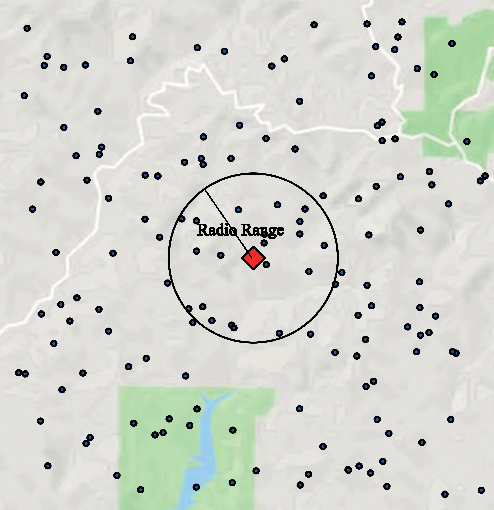
\includegraphics[width=1.7in]{./Figure/uniform.pdf}}
\vspace{0.03in}
\subfigure[Gaussian distribution]{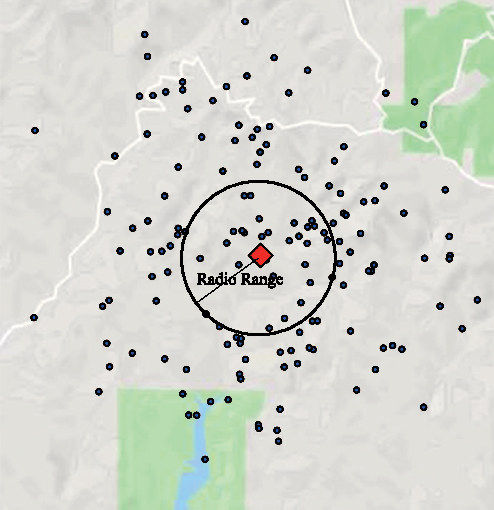
\includegraphics[width=1.7in]{./Figure/normal.pdf}}
\caption{Node deployments following uniform and Gaussian distribution.}
\label{distribution}
%\vspace{-0.2in}
\end{figure}


In order to address these challenges, we first take the distributions of nodes into consideration. As studied in \cite{wang2013gaussian}, nodes in a wireless network are likely to follow a uniform or a Gaussian distribution (as shown in Fig. \ref{distribution}), the distribution of nodes can be utilized to trigger neighbor discovery for multiple nodes. Then, we propose Alano\footnote{Alano is the god of luck in Greek mythology.}, a nearly optimal randomized algorithm for a large-scale network that achieves low discovery latency under the protocol model. Finally, we involve the duty cycle mechanism to save energy, and modify Alano for nodes that have different duty cycle constraints. Specifically, if all nodes' duty cycle are the same, such as a batch of intelligent devices have a default duty cycle setting, we call them \emph{symmetric nodes} and propose a Relaxed Difference Set based algorithm (called RDS-Alano); if nodes have different duty cycle constraints, such as a mobile phone adjusts its duty cycle by the remaining energy, we call them \emph{asymmetric nodes} and propose a Traversing Pointer based algorithm (called TP-Alano).
The contributions of the paper are summarized as follows:
\begin{itemize}
\item[1)] We utilize nodes' distribution to trigger Alano, a nearly optimal algorithm for a large-scale network that achieves low latency for discovering all neighbors;
\item[2)] In an energy-restricted large-scale network, we propose RDS-Alano for symmetric nodes and TP-Alano for asymmetric nodes. Both algorithms achieve low latency for discovering all neighbors under duty cycle mechanism that prolongs a node's lifetime;
\item[3)] We conduct extensive simulations to compare Alano with the state-of-the-art algorithms. Based on evaluation of speed (discovery latency), quality (discovery rate), scalability and robustness, Alano achieves $31.35\%$ to $ 85.25\%$ times lower discovery latency and has higher discovery rate for both symmetric nodes and asymmetric nodes, under uniform or Gaussian distribution.
\end{itemize}

The remainder of the paper is organized as follows. The coming section highlights some related works and puts forward vital problems that the existing algorithms remain. System model and basic definitions are introduced in Section \ref{sectionmodel}. We present Alano which combines nodes' distribution in Section \ref{PCN}. We propose two modified algorithms (RDS-Alano, TP-Alano) for an energy-restricted large-scale network for both symmetric and asymmetric nodes in Section \ref{EEN}. The extensive simulation results are shown in Section \ref{Evaluation} and we conclude the paper in Section \ref{Conclusion}.




% Previous version

% Paper Logic Flow
% P1-P2 Background
% P3-P6 motivation
% P7-P11 contribution
% P12 structure

%% P1:
%% Define realistic network
%% General background
%% The situation&scenario our research applies to
%The growing interest in the Internet of Things (IoT) has resulted
%in a number of wide-area deployments of wireless networks \cite{qin2014software},
%such as wireless sensor networks \cite{yick2008wireless}, mobile campus networks
%\cite{hernandez2005comparative}, mobile gaming community \cite{cunningham2002optimizing}, etc.
%All these realistic networks possess multi-hop and large-scale characteristics obviously.

%
%% P2:
%% Why NB problem is related and important to the background in P1
%% Define what is neighbor and what is neighbor discovery problem
%% A brief introduction of the existing works and explain deterministic and probabilistic with one sentence each
%Neighbor discovery is a fundamental step of constructing a wireless network, based on
%which the network can implement further applications such as routing and broadcasting.
%The core target is for each node in the network to discover the nodes in its radio sensing range
%with one-hop communication, which are called neighbors.
%A number of existing methods \cite{dutta2008practical, kandhalu2010u,
%bakht2012searchlight, sun2014hello, chen2015heterogeneous,
%wang2015blinddate, qiu2016talk, mcglynn2001birthday,
%vasudevan2009neighbor, you2011aloha, song2014probabilistic} have been proposed
%to deal with this issue, some of which are based on deterministic techniques,
%those turn on the radio with deterministic sequences,
%while others are probabilistic approaches, those turn on the radio with different probabilities.
%
%
%% P3:
%% Crucial problem:  collision issue in a partially-connected network
%% What is a practical network model and define what is a partially-connected network
%Unfortunately, despite great efforts, neighbor discovery in a realistic network remains an open problem.
%The key issue lies in the collision condition in the large-scale networks.
%In a large-scale network, each node is only able to sense the
%nodes if their Euclidean distance is no more than a given threshold
%based on received signal strength \cite{moscibroda2006complexity, wang2013gaussian, wang2015connectivity}.
%We call this multi-hop wireless network connectivity as \emph{partially-connected}.
%
%
%% P4:
%% What issues will occur, if transferring the deterministic methods to the partially-connected network
%% On the one hand,
%On the one hand, the deterministic approaches only deal with the neighbor discovery problem for two nodes.
%When transferred to multiple nodes scenario, they can not solve the collision issue when more
%than one neighbors are transmitting simultaneously.
%
%
%% P5:
%% What issues will occur, if transferring the probabilistic methods to the partially-connected network
%% On the other hand,
%On the other hand, probabilistic approaches can deal with multiple nodes discovery well but only consider
%the network is fully-connected, the topology of which is a complete graph.
%Therefore in the large-scale network where the nodes are partially-connected,
%the probability adopted in these approaches can not be desirable
%and thus can not reduce the collision efficiently.
%To our best knowledge, no relevant researches
%have focused on the neighbor discovery problem in the large-scale networks
%where nodes are partially-connected.
%
%
%% P6:
%% Summarize our initiative insight
%Our initiative insight is to take the distribution of the nodes in the network
%into fully consideration, since in a wireless network the distribution of
%nodes' deployment directly plays a vital role in determining the intrusion
%detection capability of a communication device.
%
%% P7:
%% Our solution/contribution : we propose Alano algorithm based on the distribution of nodes for the partially-connected networks
%In this paper, we propose Alano\footnote{Alano is the god of luck in Greek mythology.},
%a nearly optimal probability based algorithm to discover neighbors in large-scale networks.
%As fully studied in \cite{wang2013gaussian} , the nodes in wireless sensor networks are likely to
%follow a uniform or a Gaussian distribution as showed in Fig. \ref{distribution},
%depending on the specific network applications, which is taken into consideration of the proposed Alano algorithm.
%
%
% \begin{figure}[!t]
%\centering
%\subfigure[uniform distribution]{\includegraphics[width=1.7in]{./Figure/uniform.eps}}
%\vspace{0.03in}
%\subfigure[Gaussian distribution]{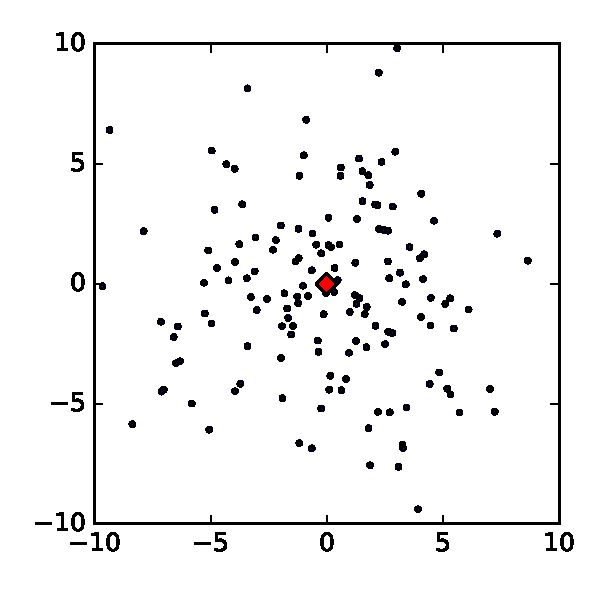
\includegraphics[width=1.7in]{./Figure/normal.eps}}
%\caption{WSN deployments following uniform and Gaussian distribution.}
%\label{distribution}
%%\vspace{-0.2in}
%\end{figure}
%
%
%% P8:
%% A special type of partially-connected networks: energy-efficient network
%In addition, among the large-scale networks, there is a special
%type named energy-efficient network \cite{jones2001survey}.
%Wireless sensor network is a typical energy-efficient network that all the sensor nodes have to maintain
%strict power budgets to attain years of lifetime\cite{dunkels2011contikimac}.
%Duty cycle mechanism, the fraction of time the radio is turned on, is
%utilized to raise the power-awareness of the nodes in the network.
%Correspondingly, the neighbor discovery process
%needs adjustments to deal with the dilemma between
%a balance of energy-efficiency and low-latency.
%
%
%% P9:
%% For energy-efficient networks, we propose RDS-Alano in global duty cycle scenario
%% and TP-Alano in the local duty cycle scenario.
%For energy-efficient networks, we design deterministic methods
%to align the wake-up time slots between the neighbors to achieve lower latency bound.
%Specifically, We propose RDS-Alano algorithm for the symmetric energy-efficient networks, where
%all the nodes share a identical duty cycle $\theta$ and TP-Alano for the
%asymmetric energy-efficient networks where each node possesses a respective duty cycle $\theta_i$.
%
%
%% P10:
%% Simulation results support our high performance
%Our simulation shows the proposed Alano algorithms
%hold significant strengths compared to the state-of-the-art methods,
%based on the evaluation of speed, quality, scalability and robustness.
%Alano achieves 31.35\% to 32.32 times lower latency
%and has higher discovery rate during the whole process of neighbor discovery,
%no matter in symmetric or asymmetric scenario and in uniform or Gaussian distribution.
%When the number of nodes increases and the network becomes denser,
%Alano still keeps its high performance.
%
%
%% P11:
%% Contribution summarize
%The main contributions of this paper are summarized as follows:
%\begin{itemize}
%\item[1)] We consider the distribution of nodes and propose Alano,
%a low-latency algorithm to achieve neighbor discovery process in a large-scale network.
%\item[2)] We propose a Relaxed Difference Set based Alano algorithm (RDS-Alano)
%to achieve low-latency neighbor discovery process in the symmetric energy-efficient networks.
%\item[3)] We propose a Traversing Pointer based Alano algorithm (TP-Alano) to
%achieve low-latency neighbor discovery process in the asymmetric energy-efficient networks.
%\end{itemize}
%
%
%% P12:
%% Remaining structure
%The remainder of the paper is organized as follows.
%The next section highlights some related work and
%puts forward some serious problems.
%Some notion definitions and the system model are given in Section \ref{sectionmodel}.
%We analyse the node's expected number of neighbors and
%propose Alano algorithm in \ref{PCN} as a foundation.
%Section \ref{EEN} describes the RDS-Alano algorithm for
%symmetric scenario and TP-Alano algorithm for asymmetric scenario
%respectively in energy-efficient networks.
%We have conducted extensive simulations, and the results are shown in Section
%\ref{Evaluation}. Finally, we conclude the paper in Section
%\ref{Conclusion}.

